
\newif\ifslides\slidestrue
%\slidesfalse

\ifslides
    \documentclass[12pt,envcountsect]{beamer}
    %\documentclass[handout]{beamer}
    \usepackage{amssymb,amsmath,url}
    \definecolor{links}{HTML}{FF0044}
    \hypersetup{colorlinks,urlcolor=links}
    \usepackage{pgfplots}
    \usepackage{pgfpages}
    \setlength{\parskip}{1ex}
    \mode<handout>{
        \usepackage{pgfpages}
        \pgfpagesuselayout{4 on 1}
        [a4paper,border shrink=5mm,landscape]
    }
\else
    \documentclass[10pt,a4paper]{article}
    \usepackage{amsthm,amssymb,amsmath,hyperref,fancyhdr,boxedminipage,graphics,color}
    \usepackage[envcountsect]{beamerarticle}
    \pagestyle{fancyplain}
    \lhead[\fancyplain{}{\thepage}]{\fancyplain{}{}}
    \cfoot{}
    \rhead[\fancyplain{}{}]{\fancyplain{}{\thepage}}
    \setlength{\parskip}{1em}
    \setlength{\parindent}{0em}
    \renewcommand{\baselinestretch}{1.2}
    \setlength{\skip\footins}{16pt}
\fi

\newif\iftitled\titledtrue

\usepackage[latin1]{inputenc}
\usepackage[english]{babel}
\usepackage{pdfpages}
\usetheme{Pittsburgh}
\usefonttheme[stillsansseriftext]{serif}
\usefonttheme{structurebold}

% Choose and set background colour
\definecolor{bgcolour}{RGB}{255,255,245}
\setbeamercolor{background canvas}{bg=bgcolour}
\setbeamercolor{example text}{fg=black}

% Set-up a custom header strip
\definecolor{headercolour}{RGB}{255,255,255}
\definecolor{bordercolour}{RGB}{255,0,68}
\definecolor{palegrey}{RGB}{180,180,180}
\definecolor{darkergrey}{RGB}{100,100,100}
\setbeamercolor{headerstrip}{fg=black,bg=white}
\setbeamercolor{border}{fg=black,bg=bordercolour}
\setbeamercolor{top strip}{fg=black,bg=palegrey}
\setbeamercolor{bottom strip}{fg=black,bg=darkergrey}
\setbeamercolor{structure}{fg=black}

%sets top border strip
\setbeamertemplate{headline}
{
  \begin{beamercolorbox}[wd=\paperwidth,ht=0ex,dp=1.2ex]{headerstrip}%
  \end{beamercolorbox}%
  \begin{beamercolorbox}[wd=\paperwidth,ht=0ex,dp=0.2ex]{top strip}%
  \end{beamercolorbox}
  \begin{beamercolorbox}[wd=\paperwidth,ht=0ex,dp=0.2ex]{border}%
  \end{beamercolorbox}
  \begin{beamercolorbox}[wd=\paperwidth,ht=0ex,dp=0.3ex]{bottom strip}%
  \end{beamercolorbox}
  \begin{beamercolorbox}[wd=\paperwidth,ht=0ex,dp=4ex]{background canvas}%
  \end{beamercolorbox}
}

%gets rid of bottom navigation bars
\setbeamertemplate{footline}
{
  \begin{beamercolorbox}[wd=\paperwidth,ht=0ex,dp=0.2ex]{top strip}%
  \end{beamercolorbox}
  \begin{beamercolorbox}[wd=\paperwidth,ht=0ex,dp=0.2ex]{border}%
  \end{beamercolorbox}
  \begin{beamercolorbox}[wd=\paperwidth,ht=0ex,dp=0.3ex]{bottom strip}%
  \end{beamercolorbox}
  \begin{beamercolorbox}[wd=\paperwidth,ht=0ex,dp=1.2ex]{headerstrip}%
  \end{beamercolorbox}
}

%gets rid of navigation symbols
\setbeamertemplate{navigation symbols}{}

%removes italics from theorems, problems etc
\setbeamertemplate{theorems}[ams style]

%makes quotes italic in beamer article mode
\mode<article>{
  \renewenvironment{quote}{\actionenv\begin{itshape}\originalquote}{\endoriginalquote\end{itshape}\endactionenv}
}

%makes line breaks work in article mode
\makeatletter
\let\beamer@@breaker\beamer@origbreak
\let\beamer@@breakercenter\beamer@origbreakcenter
\makeatother

%makes enumerate lists nice and plain
\setbeamertemplate{enumerate item}{(\roman{enumi})}

%makes frametitles etc on the left
\mode<presentation>{\setbeamertemplate{frametitle}[default][left]}


%sets up how to introduce new sections
\AtBeginSection
[
\begin{frame}
  \usebeamerfont{section title}{\bf ~\insertsection}
  \vspace{5cm}~
\end{frame}
\addtocounter{section}{-1}
]
{
\begin{frame}
  \usebeamerfont{section title}{\bf ~\insertsection}
  \vspace{5cm}~
\end{frame}
}

\AtBeginSubsection
[
\begin{frame}
  \usebeamerfont{section title}{\bf ~\insertsubsection}
    \vspace{5cm}~
\end{frame}
]
{
\begin{frame}
  \usebeamerfont{section title}{\bf ~\insertsubsection}
    \vspace{5cm}~
\end{frame}
}

\AtBeginSubsubsection
[
\begin{frame}
  \usebeamerfont{section title}{\sc ~\insertsubsubsection}
    \vspace{5cm}~
\end{frame}
]
{
\begin{frame}
  \usebeamerfont{section title}{\sc ~\insertsubsubsection}
    \vspace{5cm}~
\end{frame}
}

\newcommand{\ipause}{\pause[\thebeamerpauses]}
\newcommand{\iipause}{\pause[\thebeamerpauses+1]}

\newcommand{\R}{{\mathbb R}}
\newcommand{\N}{{\mathbb N}}
\newcommand{\Q}{{\mathbb Q}}
\newcommand{\C}{{\mathbb C}}
\newcommand{\Z}{{\mathbb Z}}
\newcommand{\uda}{\updownarrow}
\newcommand{\ov}{\overline}
\newcommand{\send}{\mathop{\rm send}\nolimits}
\newcommand{\rot}{\mathop{\rm rot}\nolimits}
\newcommand{\refl}{\mathop{\rm ref}\nolimits}
\newcommand{\sgn}{\mathop{\rm sgn}\nolimits}
\newcommand{\stab}{\mathop{\rm stab}\nolimits}
\newcommand{\odd}{\mathop{\rm odd}\nolimits}
\newcommand{\even}{\mathop{\rm even}\nolimits}
\newcommand{\swop}{\mathop{\rm swop}\nolimits}
\newcommand{\cl}{\mathop{\rm cl}\nolimits}
\newcommand{\anticl}{\mathop{\rm anticl}\nolimits}
\newcommand{\orb}{\mathop{\rm orb}\nolimits}
\newcommand{\id}{\mathop{\rm id}\nolimits}
\newcommand{\fix}{\mathop{\rm fix}\nolimits}
\newcommand{\la}{\langle}
\newcommand{\ra}{\rangle}
\newcommand{\st}{{\mbox{st}}}

\newcommand{\q}{{\bf Question. }}
\newcommand{\leadingword}[1]{\textbf{#1}}

\theoremstyle{plain}
\newtheorem{thm}[theorem]{Theorem}
\newtheorem{prop}[theorem]{Proposition}
\newtheorem{cor}[theorem]{Corollary}

\theoremstyle{definition}
\newtheorem{defn}[theorem]{Definition}
\newtheorem{defns}[theorem]{Definitions}
\newtheorem{rmk}[theorem]{Remark}
\newtheorem{rmks}[theorem]{Remarks}
\newtheorem*{eg}{Example}
\newtheorem*{egs}{Examples}
\newtheorem*{Note}{Note}
\newtheorem*{notes}{Notes}
\newtheorem{algor}[theorem]{Algorithm}
\newtheorem{gloss}[theorem]{Glossary}

%environments for indenting text
\newenvironment{intext}{\begin{center}\begin{minipage}{10cm}} {\end{minipage}\end{center}}
\newenvironment{ittext}{\begin{intext}\begin{center}\em} {\end{center}\end{intext}}
\newenvironment{boxtext}{\begin{center}\begin{boxedminipage}{10cm}\begin{center} \bf } {\end{center}\end{boxedminipage}\end{center}\smallskip}

% --Notes for students (with blanks)---------
\newenvironment{btext}{\begin{color}{white}} {\end{color}}
\newenvironment{bmfpic}[6]{\begin{color}{white}\begin{mfpic}[#1][#2]{#3}{#4}{#5}{#6}\drawcolor{white}\fillcolor{white}\tlabelcolor{white}\hatchcolor{white}\headcolor{white}\pointcolor{white}} {\end{mfpic}\end{color}}
\newcommand{\shd}{}
%------------------------

%% --Complete notes------
%\newenvironment{btext}{}{}
%\newenvironment{bmfpic}[6]{\begin{mfpic}[#1][#2]{#3}{#4}{#5}{#6}} {\end{mfpic}}
%\newcommand{\shd}{\shade[1]}
%%------------------------





\newenvironment{activity}{\vspace{1ex}\noindent\textbf{Activity.}~}{}
\newenvironment{announcement}{\begin{center}\bf\large}{\end{center}}

\begin{document}

\title{Flipped teaching in mathematics}
\author{Sam Marsh\\
University of Sheffield}
\date{August 2015}

\mode<article>{
    \iftitled\maketitle\fi
}

\mode<presentation>{
    \iftitled
        \begin{frame}
        \titlepage
        \end{frame}
    \fi
}


\begin{frame}{Flipped classrooms}\pause
Mathematician \href{http://legacyrlmoore.org/reference/burton_jones.html}{Robert Lee Moore} thought lectures `mind-dulling' over a century ago.\pause

\href{http://cft.vanderbilt.edu/guides-sub-pages/flipping-the-classroom}{`Flipped classrooms'} have been used for at least 30 years.\pause

Recent experiments blending online and classroom-based teaching \href{http://www.nabt.org/websites/institution/File/docs/Four Year Section/2012 Proceedings/Marcey & Brint.pdf}{seem promising}.
\end{frame}

\begin{frame}{Our problem}
We had stubborn attendance problems on our large first-year maths for engineers modules.\pause

A standard week had\pause
\begin{itemize}
\item two lectures ($200$ or more students);\pause
\item one problem class ($40$ students, sometimes more).\pause
\end{itemize}

We'd often see attendance taper off; some students disengaged and failed badly.
\end{frame}

\begin{frame}
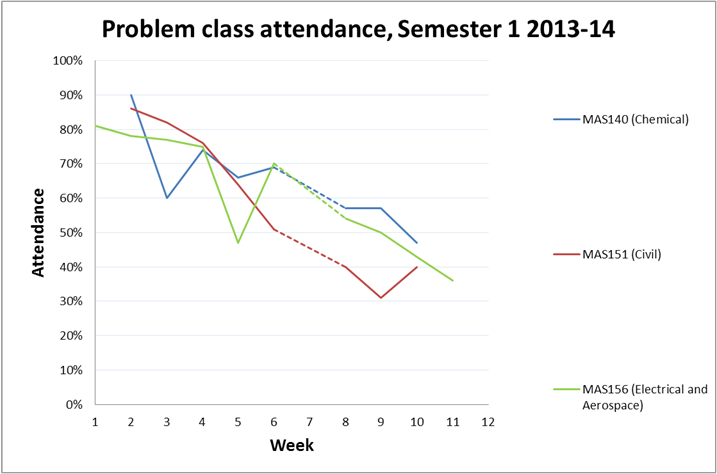
\includegraphics[width=1\textwidth]{attendance_sem1_no_MAS152.png}


\begin{itemize}
\item Week 7 was a reading week;
\item MAS156 was affected by strike action in Week 5.
\end{itemize}

\end{frame}

\begin{frame}{What to do?}\pause
We decided to scrap lectures, and focus our efforts on problem classes.\pause

Theory would be delivered with short videos, watched at home.\pause

We'd double the frequency of problem classes and change their character (more demonstration and peer discussion).
\end{frame}

\begin{frame}{What happened?}
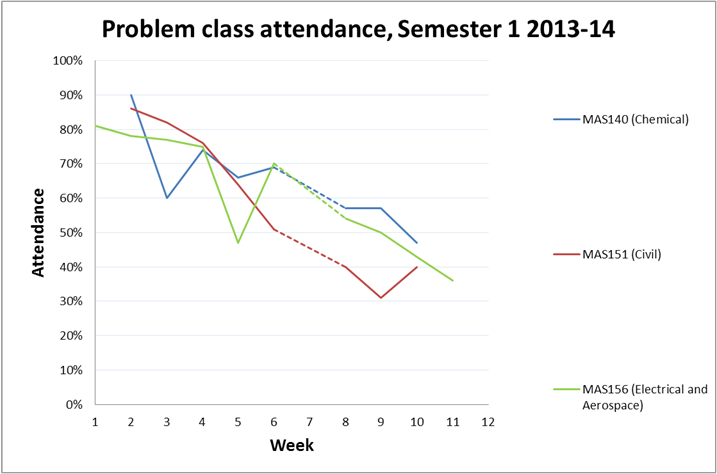
\includegraphics[width=1\textwidth]{attendance_sem1_no_MAS152.png}

\vspace{10ex}
\end{frame}

\begin{frame}{What happened?}
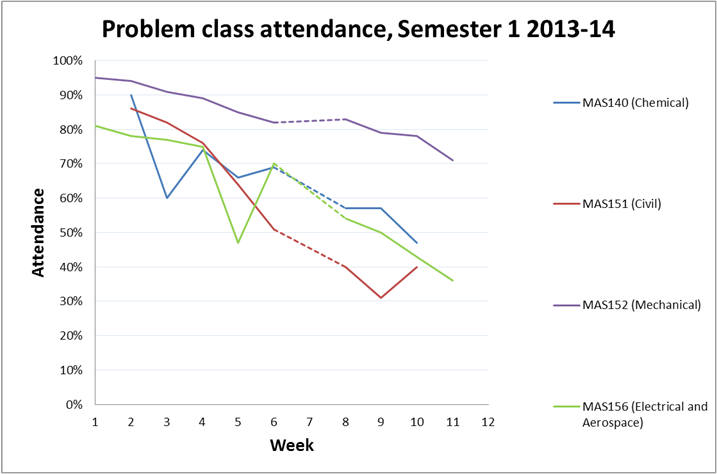
\includegraphics[width=1\textwidth]{attendance_sem1_with_MAS152.png}
\begin{itemize}
\item MAS152 is our new format module.
\end{itemize}
\end{frame}

\begin{frame}{What happened?}
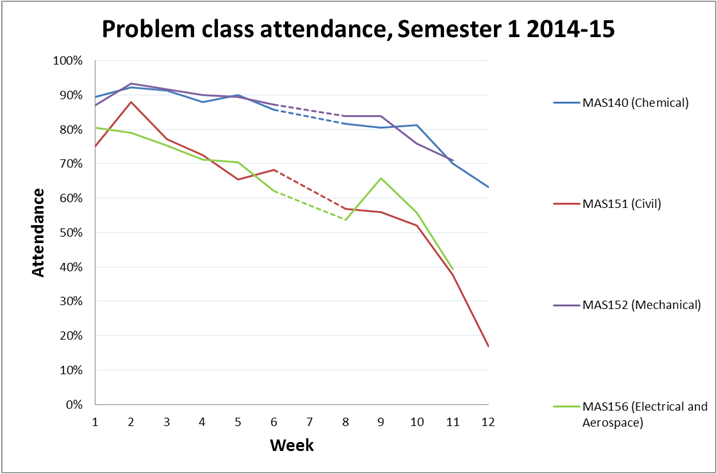
\includegraphics[width=1\textwidth]{attendance_sem1_2014_15.png}
\begin{itemize}
\item MAS140 and MAS151 now also new format.
\end{itemize}
\end{frame}

%\begin{frame}{What happened?}
%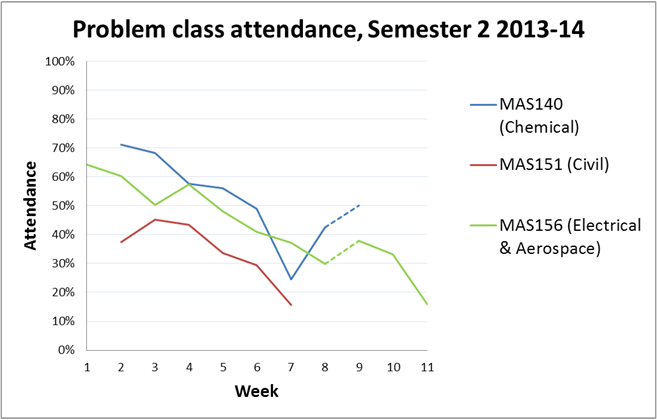
\includegraphics[width=1\textwidth]{attendance_sem2_no_MAS152.png}
%
%\vspace{10ex}
%\end{frame}
%
%\begin{frame}{What happened?}
%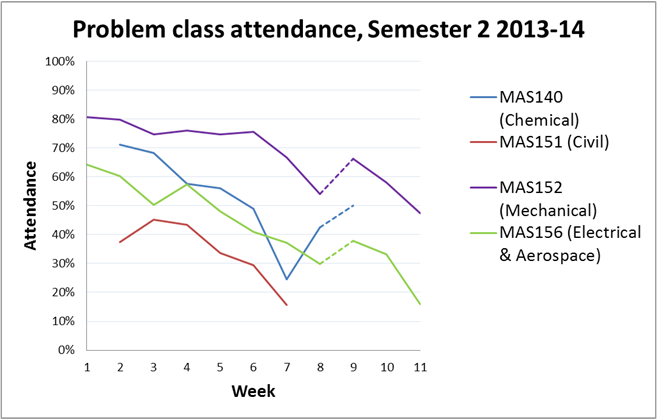
\includegraphics[width=1\textwidth]{attendance_sem2_with_MAS152.png}
%
%\vspace{10ex}
%\end{frame}


\begin{frame}{Headline findings}\pause
\begin{itemize}
\item Three times as many problem classes attended.\pause
\item Between 4--12 marks added to the average grade of a student (based on analysis of 3 years' exam data).\pause
\item Number of `bad fails' reduced by two-thirds.\pause
\item $92\%$ satisfied or very satisfied in end-of-semester questionnaires (198 responses).
\end{itemize}
\end{frame}

%\begin{frame}
%A new blended-learning format was piloted with Level 1 Mechanical engineers in 2013--14. \pause This had \pause
%\begin{itemize}
%\item 10-minute video lectures replacing face-to-face lectures;\pause
%\item short online tests following each video;\pause
%\item restructured, more interactive problem classes (and double the number);\pause
%\item online course notes and extra exercises; \pause
%\item three full-class lectures each Semester.\pause
%\end{itemize}
%(This format was devised by Nick Gurski, based on videos made by Simon Willerton and Eugenia Cheng, and with input from Stephen Beck.)
%\end{frame}

\begin{frame}{How the course works}\pause
In a standard week students complete two iterations of the cycle:\pause

log in to our video system \pause $\rightarrow$ watch 3 videos \pause $\rightarrow$ rewatch if necessary \pause $\rightarrow$ complete an online test for each \pause $\rightarrow$ attend a problem class.\pause

Demo: \url{http://goo.gl/M8WwZp}

username:\texttt{engineering}, password:\texttt{letmein}
\end{frame}

%\begin{frame}
%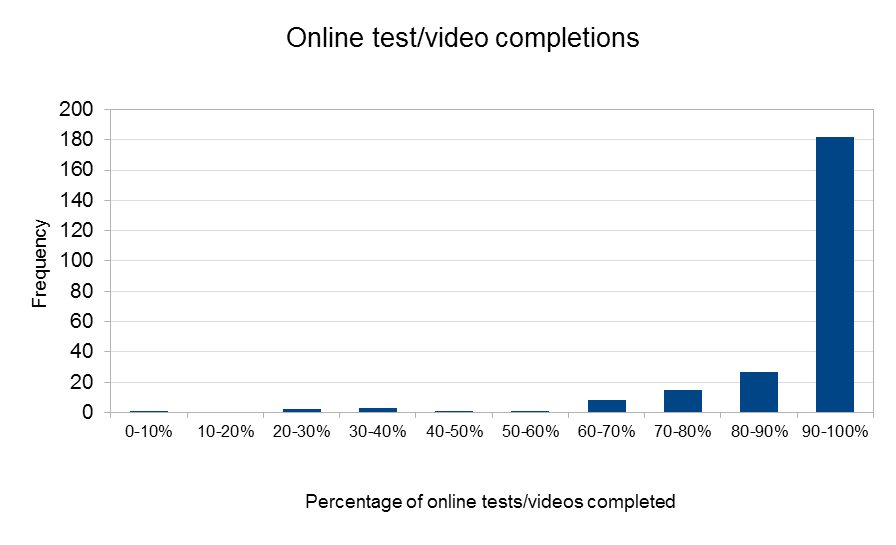
\includegraphics[width=1\textwidth]{video_completions.png}
%
%\begin{itemize}[<+->]
%\item $75\%$ of students completed $\geq 90\%$ of the videos on time.
%\item $98/240\approx 40\%$ of students completed all videos on time.
%\end{itemize}
%
%\end{frame}


\begin{frame}{Problem classes}
Each group of 40 students meets their tutor twice a week. \pause

The tutor recaps the theory from the videos, \pause encourages input on an example, \pause then sets problems and stimulates discussion.\pause

The tutor is given a lesson plan for each class.
\end{frame}

\begin{frame}
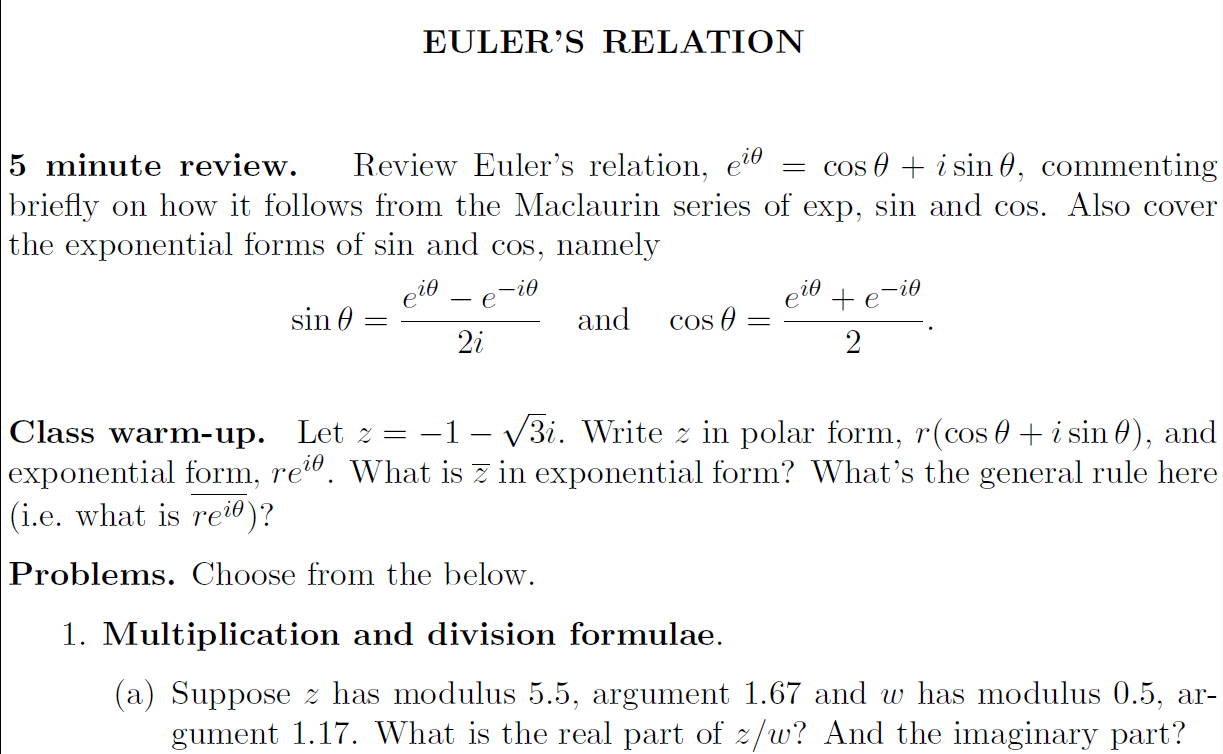
\includegraphics[width=1\textwidth]{worksheet.jpg}
\end{frame}

\begin{frame}{Speculation}
The new format seems to have solved most of our problems. \pause Why?\pause
\begin{itemize}
\item Attendance: students only attend problem classes, so are more likely to do so.\pause
\item Engagement: online tests act as a carrot for watching the videos.\pause
\item Flexibility: students choose when to watch videos, and can re-watch.\pause
\item Depth of understanding: problem classes recap the material, reinforcing learning.\pause
\item Student experience: the students are effectively in a group of 40 rather than 240 and get to know their tutor well.
\end{itemize}
\end{frame}

\begin{frame}{More information}
\begin{itemize}
\item More detail in our \href{http://sam-marsh.staff.shef.ac.uk/docs/guardian_award_application.pdf}{application for the Guardian University Awards}.
\item A Guardian discussion piece \href{http://www.theguardian.com/higher-education-network/2015/mar/31/are-lectures-the-best-way-to-teach-students}{`Are lectures the best way to teach students?'} written by me and Dr Nick Gurski.
\item Full pedagogical paper to follow.
\item The \href{http://sam-marsh.staff.shef.ac.uk/mas140_151_152?staff_view=1}{course webpage}.
\end{itemize}

\end{frame}
\end{document} 